\documentclass[12pt]{article}

%% packages
\usepackage{color,verbatim,Sweave,url,xargs,amsmath,graphicx}
\usepackage[left=0.5in, right=.5in, top=1in, bottom=.75in]{geometry}
% \usepackage{times}
\usepackage{multicol}
\usepackage{enumitem}
\usepackage{arev}
\usepackage{fancyhdr}


\setkeys{Gin}{width=0.5\linewidth}

%% new environments
\newenvironment{question}{\item}{\vfill}
\newenvironment{solution}{\comment}{\endcomment}
\newenvironment{answerlist}{\renewcommand{\labelenumi}{(\alph{enumi})}\begin{samepage}\begin{enumerate}[topsep=0pt,itemsep=-1ex,partopsep=1ex,parsep=1ex]}{\end{enumerate}\end{samepage}}
%%\newenvironment{answerlist}{\setlength{\itemsep}{0pt}\setlength{\parskip}{0pt}\renewcommand{\labelenumi}{(\alph{enumi})}\begin{multicols}{2}\begin{enumerate}}{\end{enumerate}\end{multicols}}
%% \newenvironment{answerlist}{\renewcommand{\labelenumi}{(\alph{enumi})}\begin{multicols}{2}\begin{enumerate}}{\end{enumerate}\end{multicols}}



%% paragraphs
\setlength{\parskip}{0.7ex plus0.1ex minus0.1ex}
\setlength{\parindent}{0em}

%% compatibility with pandoc
\providecommand{\tightlist}{\setlength{\itemsep}{0pt}\setlength{\parskip}{0pt}}

% %% fonts: Helvetica
% \renewcommand{\sfdefault}{phv}
% \IfFileExists{sfmath.sty}{
%   \RequirePackage{sfmath}
%   \renewcommand{\rmdefault}{phv}
% }{}



% %% headings
% \markboth{\textnormal{\bf \large Statistics Exam: \myID}}%
% {\textnormal{\bf \large Statistics Exam: \myID}}
% \pagestyle{myheadings}

\begin{document}

\pagestyle{fancy}
\fancyhf{}
\rhead{Algebra \& Trig Unit 1}
\lhead{\sc{Linear Programming}}
\chead{QUESTIONS}
\rfoot{Page \thepage}
\setlength{\headheight}{15pt}


%% title page
% \thispagestyle{empty}
% {\sf
% \textbf{\LARGE{Fusion Academy}}

% \textbf{\large{Statistics Exam \myDate \hfill Exam ID \myID}}


\vspace*{0.1cm}

\begin{flushright}
\begin{tabular}{p{14cm}}
\textbf{\large{Name:}} \hrule \\[1.5cm]
\textbf{\large{Date:}} \hrule \\[0.5cm]
% \textbf{Signature:} \hrule  \\[1.5cm]
\end{tabular}
\end{flushright}
% 
% \vspace*{1cm}

% \newpage

\begin{enumerate}

\begin{question}
A thief is filling her backpack with two types of valuable substances.
She can carry up to 40 kg, and her backpack can fit up to 15 liters.

Each bag of \(X\) has a weight of 2 kg, volume of 0.1 L, and value of
1000 thousand USD.

Each bag of \(Y\) has a weight of 0.2 kg, volume of 0.09 L, and value of
200 thousand USD.

There is no requirement to take full bags, so the thief can opt for a
fraction of a bag.

How many bags of each should the thief take to maximize her profit?
\end{question}

\begin{solution}
The thief should take 3.75 bags of \(X\) and 162.5 bags of \(Y\). We can
use linear programming to see this.

We write a weight inequality. \[2x+0.2y \le 40\] We write a volume
inequality. \[0.1x+0.09y \le 15\] We graph the two inequalities, shading
the feasible region.

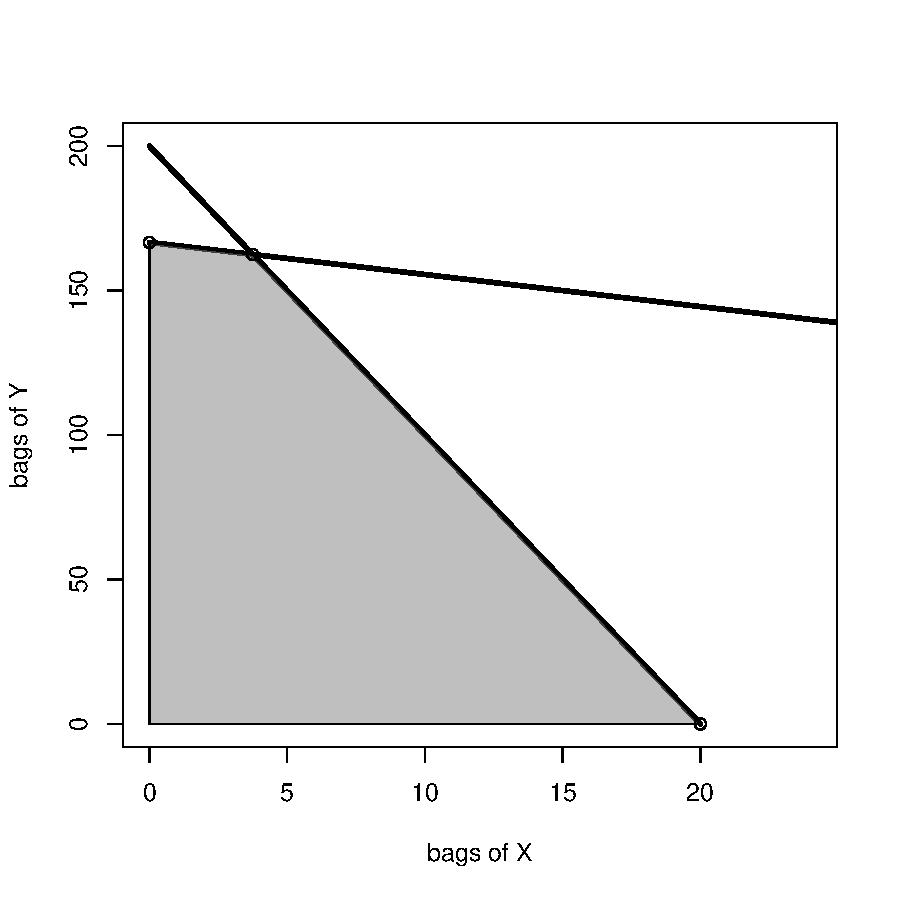
\includegraphics{unnamed-chunk-1-1.pdf}\\

There are three vertices of interest. \[(0,166.67) \] \[(3.75,162.5) \]
\[(20,0)\]

We write a profit function (the objective function).
\[P(x,y) = 1000x+200y \]

We determine the profits. \[P(0,166.67)=33333.33 \]
\[P(3.75,162.5)=36250 \] \[P(20,0)=20000 \] Thus, the thief should take
3.75 bags of \(X\) and 162.5 bags of \(Y\).
\end{solution}



\begin{question}
Determine the product of the matrix multiplication.

\[\left[\begin{matrix}-3 & 0 & 3\\1 & 6 & 6\end{matrix}\right] \cdot \left[\begin{matrix}-9 & -1\\0 & -4\\-5 & -3\end{matrix}\right]\]
\end{question}

\begin{solution}
The answer:
\[\left[\begin{matrix}12 & -6\\-39 & -43\end{matrix}\right]\]

The work:

1st row and 1st column\ldots{} \((-3)(-9)+(0)(0)+(3)(-5) = 12\)

1st row and 2nd column\ldots{} \((-3)(-1)+(0)(-4)+(3)(-3) = -6\)

2nd row and 1st column\ldots{} \((1)(-9)+(6)(0)+(6)(-5) = -39\)

2nd row and 2nd column\ldots{} \((1)(-1)+(6)(-4)+(6)(-3) = -43\)
\end{solution}


\newpage

\begin{question}
\textbf{Draw} the polynomial function \(f(x)\) shown in factored and
expanded forms. Be sure to indicate the roots, where the function is
positive or negative, and end behavior.

\[f(x) = 3 \left(x - 4\right) \left(x - 3\right)^{2} \left(x + 2\right) \left(x + 5\right)\]

\[f(x) = 3 x^{5} - 9 x^{4} - 81 x^{3} + 285 x^{2} + 234 x - 1080 \]
\end{question}

\begin{solution}
You need to consider the roots and end behavior. If a root has even
multiplicity, you need to bounce the curve off the \(x\)-axis there.

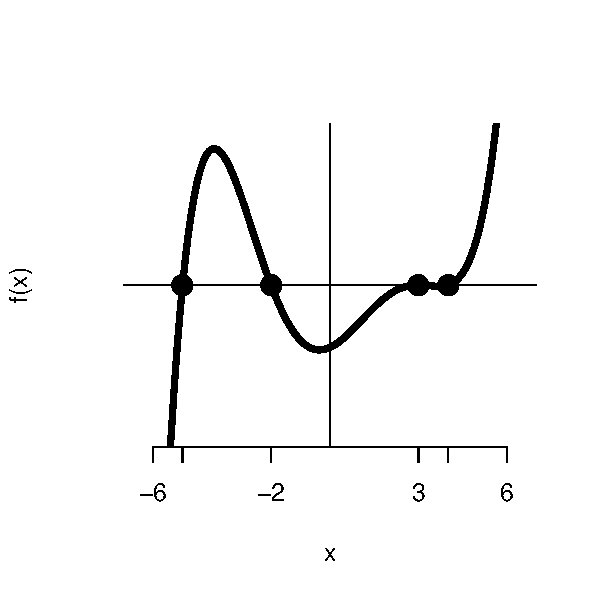
\includegraphics{unnamed-chunk-2-1-2.pdf}\\
\end{solution}



\begin{question}
Factor the polynomial function \(f(x)\) to determine the roots.

\[f(x) = - x^{3} + x^{2} + 14 x - 24 \]
\end{question}

\begin{solution}
Factor.

\[f(x) = - \left(x - 3\right) \left(x - 2\right) \left(x + 4\right)\]

The roots:

\[x|_{f(x)=0} = [-4, 2, 3]\]
\end{solution}


\newpage

\begin{question}
Solve the following system.

\[\begin{align}
- 12 x - 4 y + z&=-93\\
- 6 x - 2 y - 6 z&=-66\\
- 12 x - 4 y + 8 z&=-72
\end{align}\]
\begin{answerlist}
  \item 
  \item 
  \item 
\end{answerlist}
\end{question}

\begin{solution}
The system is undetermined. There are infinite solutions. This might be
because two planes are equivalent, or because all three planes meet in a
line, or because all three planes are equivalent.
\end{solution}



\begin{question}
A thief is filling her backpack with two types of valuable substances.
She can carry up to 35 kg, and her backpack can fit up to 25 liters.

Each bag of \(X\) has a weight of 6 kg, volume of 0.5 L, and value of
600 thousand USD.

Each bag of \(Y\) has a weight of 1 kg, volume of 1 L, and value of 1000
thousand USD.

There is no requirement to take full bags, so the thief can opt for a
fraction of a bag.

How many bags of each should the thief take to maximize her profit?
\end{question}

\begin{solution}
The thief should take 1.82 bags of \(X\) and 24.09 bags of \(Y\). We can
use linear programming to see this.

We write a weight inequality. \[6x+1y \le 35\] We write a volume
inequality. \[0.5x+1y \le 25\] We graph the two inequalities, shading
the feasible region.

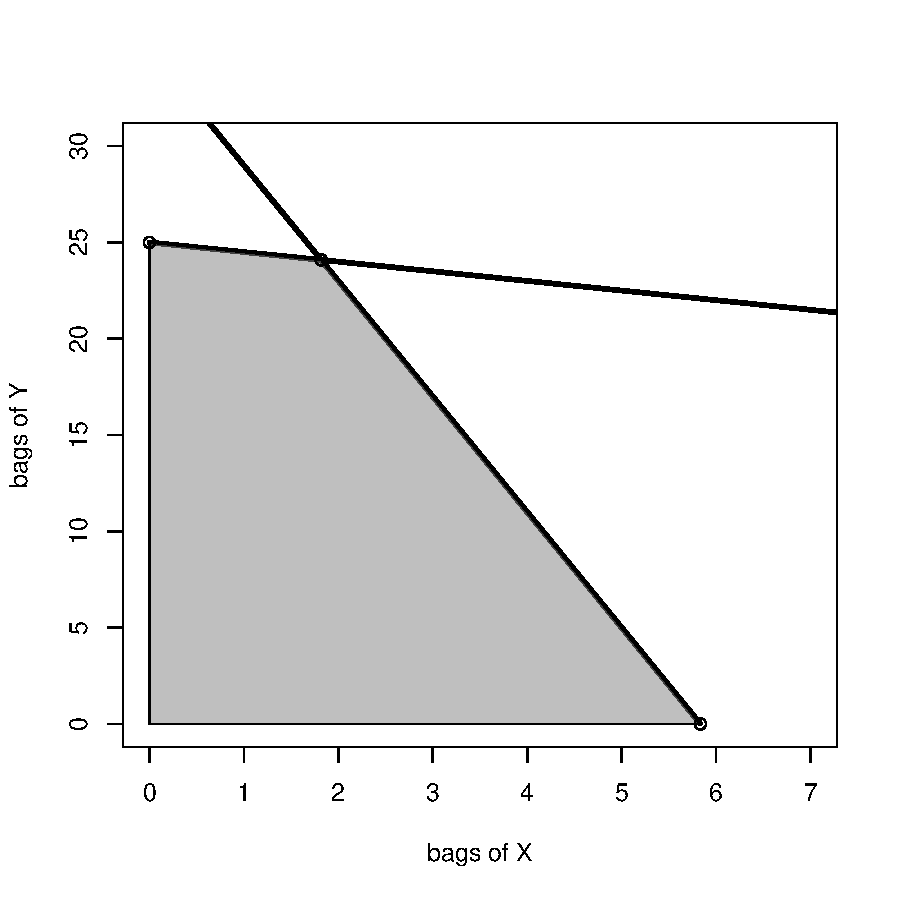
\includegraphics{unnamed-chunk-1-1-6.pdf}\\

There are three vertices of interest. \[(0,25) \] \[(1.82,24.09) \]
\[(5.83,0)\]

We write a profit function (the objective function).
\[P(x,y) = 600x+1000y \]

We determine the profits. \[P(0,25)=25000 \] \[P(1.82,24.09)=25181.82 \]
\[P(5.83,0)=3500 \] Thus, the thief should take 1.82 bags of \(X\) and
24.09 bags of \(Y\).
\end{solution}


\end{enumerate}

\newpage

\renewenvironment{question}{\comment}{\endcomment}
\renewenvironment{solution}{\item}{\vfill}


\chead{SOLUTIONS}

\begin{enumerate}

\begin{question}
A thief is filling her backpack with two types of valuable substances.
She can carry up to 40 kg, and her backpack can fit up to 15 liters.

Each bag of \(X\) has a weight of 2 kg, volume of 0.1 L, and value of
1000 thousand USD.

Each bag of \(Y\) has a weight of 0.2 kg, volume of 0.09 L, and value of
200 thousand USD.

There is no requirement to take full bags, so the thief can opt for a
fraction of a bag.

How many bags of each should the thief take to maximize her profit?
\end{question}

\begin{solution}
The thief should take 3.75 bags of \(X\) and 162.5 bags of \(Y\). We can
use linear programming to see this.

We write a weight inequality. \[2x+0.2y \le 40\] We write a volume
inequality. \[0.1x+0.09y \le 15\] We graph the two inequalities, shading
the feasible region.

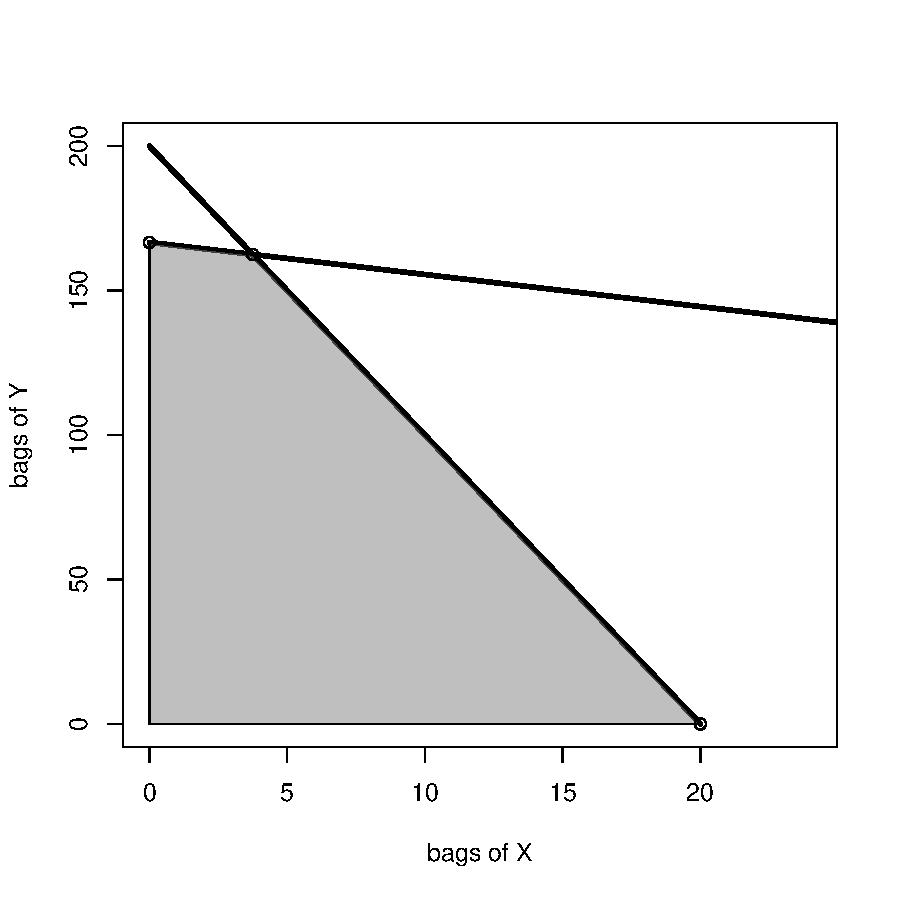
\includegraphics{unnamed-chunk-1-1.pdf}\\

There are three vertices of interest. \[(0,166.67) \] \[(3.75,162.5) \]
\[(20,0)\]

We write a profit function (the objective function).
\[P(x,y) = 1000x+200y \]

We determine the profits. \[P(0,166.67)=33333.33 \]
\[P(3.75,162.5)=36250 \] \[P(20,0)=20000 \] Thus, the thief should take
3.75 bags of \(X\) and 162.5 bags of \(Y\).
\end{solution}



\begin{question}
Determine the product of the matrix multiplication.

\[\left[\begin{matrix}-3 & 0 & 3\\1 & 6 & 6\end{matrix}\right] \cdot \left[\begin{matrix}-9 & -1\\0 & -4\\-5 & -3\end{matrix}\right]\]
\end{question}

\begin{solution}
The answer:
\[\left[\begin{matrix}12 & -6\\-39 & -43\end{matrix}\right]\]

The work:

1st row and 1st column\ldots{} \((-3)(-9)+(0)(0)+(3)(-5) = 12\)

1st row and 2nd column\ldots{} \((-3)(-1)+(0)(-4)+(3)(-3) = -6\)

2nd row and 1st column\ldots{} \((1)(-9)+(6)(0)+(6)(-5) = -39\)

2nd row and 2nd column\ldots{} \((1)(-1)+(6)(-4)+(6)(-3) = -43\)
\end{solution}



\begin{question}
\textbf{Draw} the polynomial function \(f(x)\) shown in factored and
expanded forms. Be sure to indicate the roots, where the function is
positive or negative, and end behavior.

\[f(x) = 3 \left(x - 4\right) \left(x - 3\right)^{2} \left(x + 2\right) \left(x + 5\right)\]

\[f(x) = 3 x^{5} - 9 x^{4} - 81 x^{3} + 285 x^{2} + 234 x - 1080 \]
\end{question}

\begin{solution}
You need to consider the roots and end behavior. If a root has even
multiplicity, you need to bounce the curve off the \(x\)-axis there.

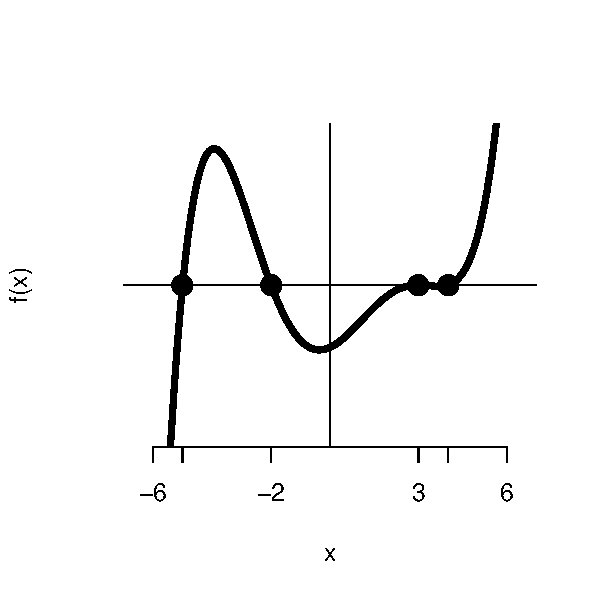
\includegraphics{unnamed-chunk-2-1-2.pdf}\\
\end{solution}



\begin{question}
Factor the polynomial function \(f(x)\) to determine the roots.

\[f(x) = - x^{3} + x^{2} + 14 x - 24 \]
\end{question}

\begin{solution}
Factor.

\[f(x) = - \left(x - 3\right) \left(x - 2\right) \left(x + 4\right)\]

The roots:

\[x|_{f(x)=0} = [-4, 2, 3]\]
\end{solution}



\begin{question}
Solve the following system.

\[\begin{align}
- 12 x - 4 y + z&=-93\\
- 6 x - 2 y - 6 z&=-66\\
- 12 x - 4 y + 8 z&=-72
\end{align}\]
\begin{answerlist}
  \item 
  \item 
  \item 
\end{answerlist}
\end{question}

\begin{solution}
The system is undetermined. There are infinite solutions. This might be
because two planes are equivalent, or because all three planes meet in a
line, or because all three planes are equivalent.
\end{solution}



\begin{question}
A thief is filling her backpack with two types of valuable substances.
She can carry up to 35 kg, and her backpack can fit up to 25 liters.

Each bag of \(X\) has a weight of 6 kg, volume of 0.5 L, and value of
600 thousand USD.

Each bag of \(Y\) has a weight of 1 kg, volume of 1 L, and value of 1000
thousand USD.

There is no requirement to take full bags, so the thief can opt for a
fraction of a bag.

How many bags of each should the thief take to maximize her profit?
\end{question}

\begin{solution}
The thief should take 1.82 bags of \(X\) and 24.09 bags of \(Y\). We can
use linear programming to see this.

We write a weight inequality. \[6x+1y \le 35\] We write a volume
inequality. \[0.5x+1y \le 25\] We graph the two inequalities, shading
the feasible region.

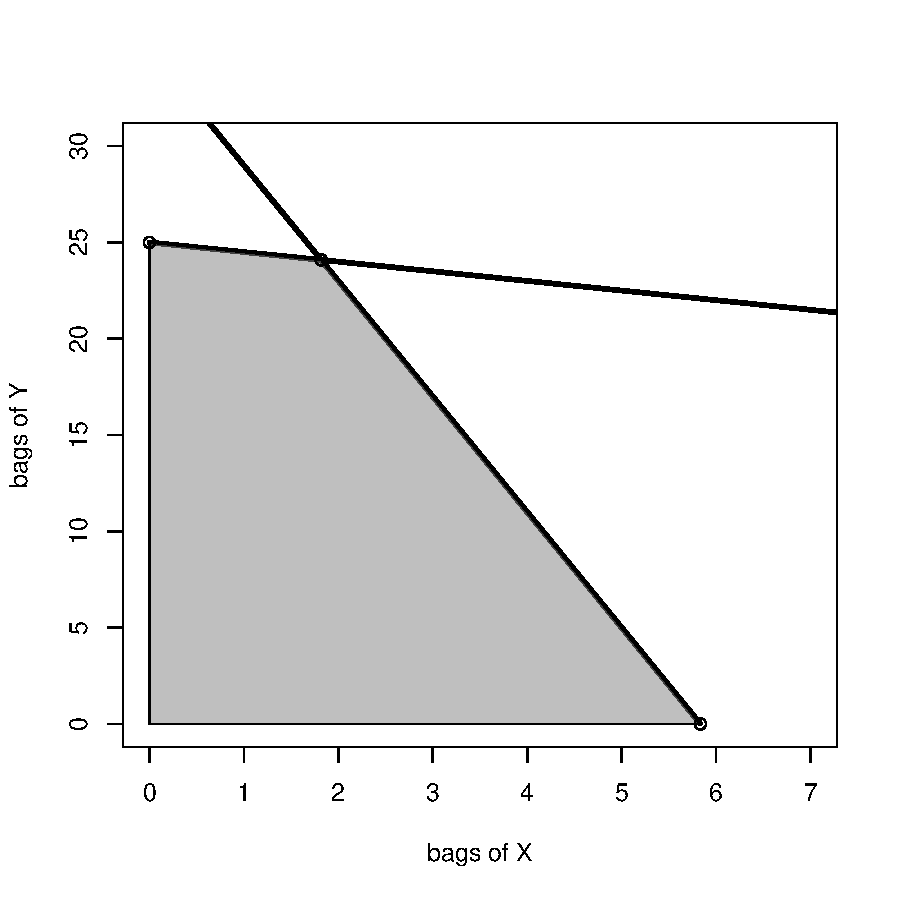
\includegraphics{unnamed-chunk-1-1-6.pdf}\\

There are three vertices of interest. \[(0,25) \] \[(1.82,24.09) \]
\[(5.83,0)\]

We write a profit function (the objective function).
\[P(x,y) = 600x+1000y \]

We determine the profits. \[P(0,25)=25000 \] \[P(1.82,24.09)=25181.82 \]
\[P(5.83,0)=3500 \] Thus, the thief should take 1.82 bags of \(X\) and
24.09 bags of \(Y\).
\end{solution}


\end{enumerate}

\end{document}
